\section{Khảo sát sự biến thiên và vẽ đồ thị hàm số}
\subsection{Đề 1}
\Opensolutionfile{ans}[ans/ans-2-B4]
\caulc
\begin{ex}%[2D1H5-7]
	Số điểm có toạ độ nguyên trên đồ thị hàm số $y=\dfrac{2x+4}{x-1}$ là
	\choice
	{\True $8$}
	{$7$}
	{$9$}
	{$6$}
	\loigiai{
		$y=2+\dfrac{6}{x-1}$, $y\in \mathbb{Z}\Leftrightarrow x-1$ là ước nguyên của $6$.
		$$x-1\in \left\{\pm 1; \; \pm 2;\; \pm 3;\pm 6\right\}\Rightarrow x\in \left\{-5; \;-2;\;-1;\; 0;\; 2;\; 3;\; 4;\; 7\right\}.$$
		Vậy có $8$ điểm có toạ độ nguyên trên đồ thị. 
	} 
\end{ex}
%%%==============EX_2============%%%
\begin{ex}%[2D1H5-7]
	Đồ thị hàm số $y=\dfrac{x-1}{-x+2}$ có tâm đối xứng là điểm có tọa độ
	\choice
	{\True $I(2;-1)$}
	{$I(-2;1)$}
	{$I(2;1)$}
	{$I(2;-1)$}
	\loigiai{
		Tâm đối xứng của đồ thị hàm số $y=\dfrac{x-1}{-x+2}$ là giao điểm hai tiệm cận của nó.\\
		Mà đồ thị hàm số có tiệm cận đứng  $x=2$ và tiệm cận ngang $y=-1$. 
	} 
\end{ex}
%%%==============EX_3============%%%
\begin{ex}%[2D1H5-7]
	\immini{Đồ thị như hình vẽ là  của hàm số 
		\choice
		{$y=\dfrac{x-1}{-x-1}$}
		{\True $y=\dfrac{x+1}{x-1}$}
		{$y=\dfrac{x+1}{-x+1}$}
		{$y=\dfrac{x-1}{x+1}$}
	}{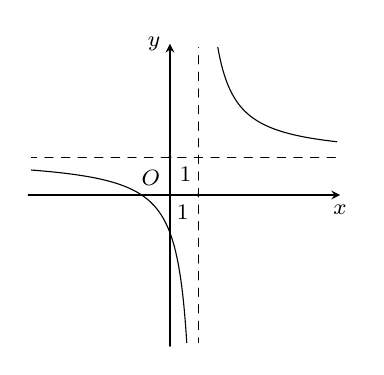
\begin{tikzpicture}[scale=0.6,xscale=0.6,yscale=0.8,>=stealth, font=\footnotesize, line join=round, line cap=round]
			\def\a{1} \def\b{1} \def\c{1} \def\d{-1} % Hệ số
			\def\xmin{-5} \def\xmax{6}
			\def\ymin{-4} \def\ymax{4}
			% 	 	\draw[color=gray!50,dashed] (\xmin,\ymin) grid (\xmax,\ymax);
			\draw[->] (\xmin,0)--(\xmax,0) node [below]{$x$};
			\draw[->] (0,\ymin)--(0,\ymax) node [left]{$y$};
			\node at (0,0) [above left]{$O$};
			\clip (\xmin+0.1,\ymin+0.1) rectangle (\xmax-0.1,\ymax-0.1);
			\draw[smooth,samples=300,domain=\xmin:(-\d/\c-0.1)] plot(\x,{(\a*(\x)+\b)/(\c*(\x)+\d)});
			\draw[smooth,samples=300,domain=(-\d/\c+0.1:\xmax)] plot(\x,{(\a*(\x)+\b)/(\c*(\x)+\d)});
			\draw[dashed] (-\d/\c,\ymin)--(-\d/\c,\ymax);
			\draw[dashed] (\xmin,\a/\c)--(\xmax,\a/\c);
			\draw[fill=black]
			(0,1)node[below right]{$1$}circle(1pt)
			(1,0)node[below left]{$1$}circle(1pt)
			
			;
	\end{tikzpicture}}
	\loigiai{
		Dựa vào đồ thị ta có có tiệm cận đứng là $x=1$ và tiệm cận ngang là $y=1$ nên hàm số thỏa mãn là $y=\dfrac{x+1}{x-1}$.
	}
\end{ex}
\begin{ex}%[2D1H5-7]
	\immini{Đồ thị như hình vẽ là của hàm số 
		\choice
		{$y=x^3-x^2+x+1$}
		{\True $y=x^3-3x^2+3$}
		{$y=x^3+3x^2+3x+1$}
		{$y=x^2+2x+1$}
	}{\begin{tikzpicture}[scale=0.6,>=stealth, font=\footnotesize, line join=round, line cap=round]
			\def\a{1} \def\b{-3} \def\c{0} \def\d{3} % Hệ số
			\def\xmin{-2} \def\xmax{5}
			\def\ymin{-2} \def\ymax{4} 
			%\draw[color=gray!50,dashed] (\xmin,\ymin) grid (\xmax,\ymax); 
			\draw[->] (\xmin,0)--(\xmax,0) node [below]{$x$};
			\draw[->] (0,\ymin)--(0,\ymax) node [left]{$y$};
			\node at (0,0) [below left]{$O$};
			\clip (\xmin+0.1,\ymin+0.1) rectangle (\xmax-0.5,\ymax-0.1);
			\draw[smooth,samples=300] plot(\x,{\a*(\x)^3+\b*(\x)^2+\c*(\x)+\d});
	\end{tikzpicture}}
	\loigiai{
		Dựa vào đồ thị ta có hàm số đã cho là hàm số bậc 3 và có 2 cực trị nên $y=x^3-3x^2+3$.
	}
\end{ex}
\begin{ex}%[2D1H5-7]
	\immini{Đường cong ở hình bên là đồ thị của hàm số $y=\dfrac{a x+b}{c x+d}$. Mệnh đề nào dưới đây đúng?
		\choice
		{$y'<0$, $\forall x\ne2$} 
		{$y'<0$, $\forall x\ne-1$}
		{$y'>0$, $\forall x\ne 2$}
		{\True $y'>0$, $\forall x\ne- 1$}}{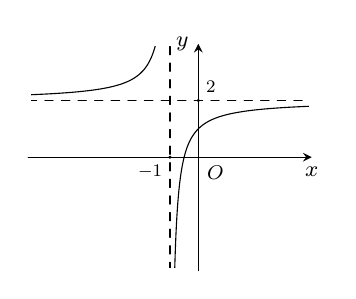
\begin{tikzpicture}[scale=0.6,xscale=0.6,yscale=0.6,>=stealth, font=\footnotesize, line join=round, line cap=round]
			\def\a{2} \def\b{1} \def\c{1} \def\d{1} % Hệ số
			\def\xmin{-6} \def\xmax{4}
			\def\ymin{-4} \def\ymax{4}
			% 	 	\draw[color=gray!50,dashed] (\xmin,\ymin) grid (\xmax,\ymax);
			\draw[->] (\xmin,0)--(\xmax,0) node [below]{$x$};
			\draw[->] (0,\ymin)--(0,\ymax) node [left]{$y$};
			\node at (0,0) [below right,scale=0.9]{$O$};
			\clip (\xmin+0.1,\ymin+0.1) rectangle (\xmax-0.1,\ymax-0.1);
			\draw[smooth,samples=300,domain=\xmin:(-\d/\c-0.1)] plot(\x,{(\a*(\x)+\b)/(\c*(\x)+\d)});
			\draw[smooth,samples=300,domain=(-\d/\c+0.1:\xmax)] plot(\x,{(\a*(\x)+\b)/(\c*(\x)+\d)});
			\draw[dashed] (-\d/\c,\ymin)--(-\d/\c,\ymax);
			\draw[dashed] (\xmin,\a/\c)--(\xmax,\a/\c);
			\draw[fill=black](-1,0)node[below left,scale=0.8]{$-1$}circle(1pt)
			(0,2)node[above right,scale=0.8]{$2$}circle(1pt)
			;
	\end{tikzpicture}}
	\loigiai{
		Dựa vào đồ thị ta có hàm số đồng biến trên $\mathbb{R}\setminus  \{-1\}$ nên	$y'>0$, $\forall x\ne- 1$.
	}
\end{ex}
%%%==============EX_4============%%%
\begin{ex}%[2D1H5-7]
	Bảng biến thiên sau là  của hàm số 
	\begin{center}
		
\begin{tikzpicture}
			\tkzTabInit[nocadre=false,lgt=1.2,espcl=2.5,deltacl=0.6]
			{$x$ /0.6, $y'$ /0.6, $y$ /2}
			{$-\infty$,$0$,$2$,$+\infty$}
			\tkzTabLine{ ,+,0,-,0,+, }
			\tkzTabVar{-/$-\infty$,+/$-1$,-/$-5$,+/$+\infty$}
		\end{tikzpicture}
	\end{center}
	\choice
	{$ y=-x^3-3x-2 $}
	{\True $ y=x^3-3x^2-1 $}
	{$ y=-x^3+3x^2-2 $}
	{$ y=-x^3+3x^2-1 $}
	\loigiai{
		\textbf{Cách 1}: Nhìn vào bảng biến thiên ta thấy $ a > 0 $ nên hàm số cần tìm là $ y=x^3-3x^2-1 $.\\
		\textbf{Cách 2}: Ta có $ y'=3x^2-6x \Rightarrow y' = 0\Leftrightarrow \hoac{ & x=0 \\  & x=2. }$\\
		BBT:
		\begin{center}
			
\begin{tikzpicture}
				\tkzTabInit[nocadre=false,lgt=1.2,espcl=2.5,deltacl=0.6]
				{$x$ /0.6, $y'$ /0.6, $y$ /2}
				{$-\infty$,$0$,$2$,$+\infty$}
				\tkzTabLine{ ,+,0,-,0,+, }
				\tkzTabVar{-/$-\infty$,+/$-1$,-/$-5$,+/$+\infty$}
			\end{tikzpicture}
		\end{center}
	}
\end{ex}
%%%==============EX_5============%%%
\begin{ex}%[2D1H5-7]
	\immini{
		Xác định các hệ số $a, b, c$ để đồ thị hàm số $y=\dfrac{ax-1}{bx+c}$ có đồ thị hàm số như hình vẽ bên:
		\choice
		{$a=2,b=2,c=-1$}
		{$a=2,b=-1,c=1$}
		{$a=2,b=1,c=1$}
		{\True $a=2,b=1,c=-1$}}
	{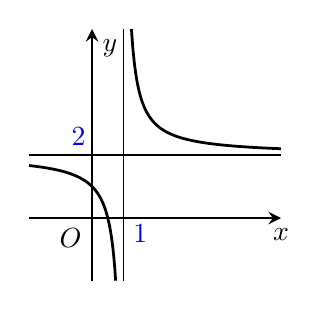
\begin{tikzpicture}[>=stealth,scale=0.4]
			\draw[->,line width = 1pt] (-2,0)--(0,0) node[below left]{$O$}--(6,0) node[below]{$x$}; %Ox
			\draw[->,line width = 1pt] (0,-2) --(0,6) node[below right]{$y$}; %Oy
			\foreach \x in {1}{\draw (\x,-.1)--(\x,.1) node[below right,blue]{$\x$};}%Oy
			
			\foreach \y in {2}{\draw[-] (-.1,\y)--(.1,\y) node[above left,blue]{$\y$};}%Oy
			\draw [black, line width = 1pt]%
			plot[domain=-2:0.75, samples=100] (\x, {((\x)*2-1)/(\x-1)});
			\draw [black, line width = 1pt]%
			plot[domain=1.25:6, samples=100] (\x, {((\x)*2-1)/(\x-1)});
			\draw [domain=-2:6] plot (\x,{2}); %TCN
			\draw [-] (1,6)--(1,-2); %TCD
			
	\end{tikzpicture}}
	\loigiai{
		\textbf{Phương pháp:}\\
		Dựa vào đồ thị hàm số để nhận xét và đưa ra công thức đúng về đồ thị hàm số, từ đó suy ra các giá trị $a, b, c$.\\
		\textbf{Cách giải:}\\
		Dựa vào đồ thị hàm số ta thấy đồ thị hàm số có tiệm cận đứng là $y=2\Rightarrow y=\dfrac{a}{b}=2$.\\
		Đồ thị hàm số đi qua điểm $\left(0;1\right)$ nên $-\dfrac{1}{c}=1\Rightarrow c=-1$.\\
		Mặt khác $-\dfrac {c}{b}=1\Rightarrow b=1$ suy ra $a=2$.
	}
\end{ex}
%%%==============EX_6============%%%
\begin{ex}%[2D1H5-7]
	\immini{Đường cong ở hình bên là đồ thị của hàm số $y=ax^3+b x^2+cx+d$. Khi đó phương trình $y'=0$
		\choice
		{có hai nghiệm $x=0$ và $x=1$}
		{có hai nghiệm $x=\pm1$}
		{vô nghiệm}
		{\True có một nghiệm kép $x=1$}}{\begin{tikzpicture}[scale=0.9,>=stealth, font=\footnotesize, line join=round, line cap=round]
			\def\a{1} \def\b{-3} \def\c{3} \def\d{-1} % Hệ số
			\def\xmin{-2} \def\xmax{3}
			\def\ymin{-2} \def\ymax{2} 
			%	\draw[color=gray!50,dashed] (\xmin,\ymin) grid (\xmax,\ymax); 
			\draw[->] (\xmin,0)--(\xmax,0) node [below]{$x$};
			\draw[->] (0,\ymin)--(0,\ymax) node [left]{$y$};
			\node at (0,0) [below left]{$O$};
			\clip (\xmin+0.1,\ymin+0.1) rectangle (\xmax-0.5,\ymax-0.1);
			\draw[smooth,samples=300] plot(\x,{\a*(\x)^3+\b*(\x)^2+\c*(\x)+\d});
			%	\draw[dashed](1,0)|-(0,-1);
			\draw(0,-1)node[left]{$-1$}circle(1pt) (1,0)node[above]{$1$}circle(1pt);
	\end{tikzpicture}}
	\loigiai{
		Dựa vào hình dáng đồ thị ta có $y'=0$ có đúng một nghiệm $x=1$.
	}
\end{ex}
%%%==============EX_7============%%%%[2D1H5-7]
\begin{ex}%[2D1H5-7]
	\immini{ Đường cong sau đây là đồ thị hàm số nào?
		\choice
		{$y=-x^3-3x+2$}
		{$y=\dfrac{x-1}{x}$}
		{\True $y=\dfrac{-x^2}{x+1}$}
		{$y=x^3+3x-2$}}
	{ \begin{tikzpicture}[line cap=butt,line join=miter,>=stealth,scale=0.5,font=\tiny]
			\tikzset{declare function={xmin=-6.2;xmax=4.8;ymin=-4.6;ymax=7.8;},
				smooth,samples=450}
			\draw[->] (xmin,0)--(xmax,0) node[shift={(0:7pt)}]{$ x $};
			\draw[->] (0,ymin)--(0,ymax) node[shift={(90:7pt)}]{$ y $};
			\fill (0,0) node[shift={(140:5pt)}]{$O$};
			\clip (xmin,ymin-.7) rectangle (xmax,ymax);
			\foreach\i in {-2,2}{\draw(\i,1.5pt)--(\i,-1.5pt)node[below]{$\i$};}
			\foreach\j in {-2,2,4}{\draw(-1.5pt,\j)--(1.5pt,\j) node[right]{$\j$};}
			\def\f(#1){(-(#1)^2)/((#1)+1)} % Hàm số
			\def\q(#1){(-(#1)+1)} % Tiệm cận xiên
			\def\a{0}
			\def\b{-2}
			\pgfmathsetmacro\fa{\f(\a)}
			\pgfmathsetmacro\fb{\f(\b)}
			\draw[samples=250] plot[domain=-7.4:-1.1] (\x,{\f(\x)});
			\draw[samples=250] plot[domain=-0.9:15] (\x,{\f(\x)});
			\draw[] plot [domain=-7.4:7] (\x,{\q(\x)}) ;
			\draw[] (-1,ymin)--(-1,ymax) node[sloped,pos=0.9,below] {$x=-1$};
			\foreach\x/\y in {\a/\fa,\b/\fb}{
				\draw[dashed] (\x,0)|-(0,\y);}
			\foreach\x/\y in {\a/\fa,\b/\fb}{\fill[white,draw=black] (\x,\y) circle (1pt);}
			%	\fill[white,draw=black] (-1,2) circle (1pt) node[text=black,shift={(14pt,5pt)}] {$I $};
			%	\node at (-1,-5) [right,fill=white,font=\footnotesize]{\it Hình LT $5$};
	\end{tikzpicture}}
	\loigiai
	{Dựa vào hình vẽ, đồ thị hàm số có tiệm cận xiên nên hàm số cần tìm là
		$y=\dfrac{-x^2}{x+1}$.
	}
\end{ex}
%%%==============EX_8============%%%
\begin{ex}%[2D1H5-7]
	\immini{
		Bảng biến thiên ở hình vẽ  là của hàm số 
		\choice
		{\True $ y=\dfrac{x+1}{x-1} $}
		{$ y=\dfrac{x+2}{x-1} $}
		{$ y=\dfrac{x+1}{1-x} $}
		{$ y=\dfrac{2x+1}{2x+3} $}
	}{
		
\begin{tikzpicture}
			\tkzTabInit[nocadre=false,lgt=1.2,espcl=2.5,deltacl=0.6]
			{$x$/0.6,$y'$/0.6,$y$/2}
			{$-\infty$,$1$,$+\infty$}
			\tkzTabLine{ ,-,d,-,}
			\tkzTabVar{+/$1$,-D+/$-\infty$/$+\infty$,-/$1$}
		\end{tikzpicture}
	}
	\loigiai{
		Đồ thị hàm số có tiệm cận đứng $ x=1 $, tiệm cận ngang $ y=1 $ và nghịch biến trên mỗi khoảng xác định.\\
		Xét $ y=\dfrac{x+1}{x-1} $ có\\
		$ \lim\limits_{x\to -\infty}y=1$; $\lim\limits_{x\to +\infty}y=1 $ nên $ y=1 $ là tiệm cận ngang.\\
		$ \lim\limits_{x\to 1^{+}}y=+\infty $; $ \lim\limits_{x\to 1^{-}}y=-\infty $ nên $ x=1 $ là tiệm cận đứng.\\
		Lại có $ y'=-\dfrac{2}{(x-1)^{2}}<0 $ nên $ y=\dfrac{x+1}{x-1} $ nghịch biến trên mỗi khoảng xác định, do đó bảng biến thiên trên là của hàm số $ y=\dfrac{x+1}{x-1} $.
	}
\end{ex}
%%%==============EX_9============%%%
\begin{ex}%[2D1H5-7]
	Đồ thị của hàm số $y=\dfrac{x-2}{x+1}$ là 	
	\choice
	{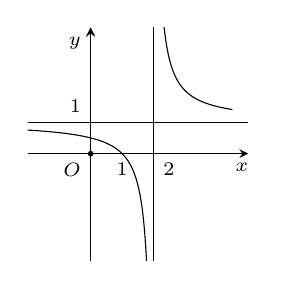
\begin{tikzpicture}[>=stealth,scale=0.4]
			\clip(-2,-3.4) rectangle (6,4);
			\draw[->,color=black] (-2,0.) -- (5,0.);
			\foreach \x in {1,2} 
			\draw[->,color=black] (0.,-4) -- (0.,4);
			\draw (2,-5)--(2,5) (-5,1)--(5,1);
			\draw[smooth,samples=100,domain=-4.5:1.9] plot(\x,{(\x-1)/(\x-2)});
			\draw[smooth,samples=100,domain=2.1:4.5] plot(\x,{(\x-1)/(\x-2)});
			\draw (0,1) node[above left] {\scriptsize $1$};
			\draw (1,0) node[below] {\scriptsize $1$};
			\draw (2,0) node[below right] {\scriptsize $2$};
			\draw (4.8,0) node[below] {\scriptsize $x$};
			\draw (0,3.5) node[left] {\scriptsize $y$};
			\draw[fill=black] (0,0) circle (2pt) node[below left] {\scriptsize $O$};
	\end{tikzpicture}}
	{\begin{tikzpicture}[>=stealth,scale=0.4]
			\clip(-5,-3) rectangle (6,5);
			\draw[->,color=black] (-5,0.) -- (3,0.);
			\draw[->,color=black] (0.,-3.4) -- (0.,5);
			\draw (-1,-5)--(-1,5) (-5,2)--(3,2);
			\draw[smooth,samples=100,domain=-4.5:-1.1] plot(\x,{(2*\x-2)/(\x+1)});
			\draw[smooth,samples=100,domain=-0.9:3] plot(\x,{(2*\x-2)/(\x+1)});
			\draw (0,2) node[above right] {\scriptsize $2$};
			\draw (1,0) node[below] {\scriptsize $2$};
			\draw (0,-2) node[right] {\scriptsize $-2$};
			\draw (3,0) node[below] {\scriptsize $x$};
			\draw (0,4.5) node[right] {\scriptsize $y$};
			\draw[fill=black] (0,0) circle (2pt) node[below left] {\scriptsize $O$};
	\end{tikzpicture}}
	{\True 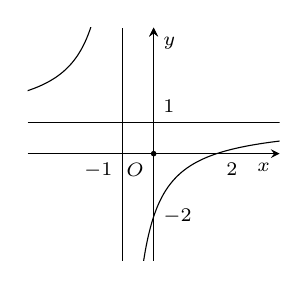
\begin{tikzpicture}[>=stealth,scale=0.4]
			\clip(-4,-3.4) rectangle (4,4);
			\draw[->,color=black] (-4,0.) -- (4,0.);
			\foreach \x in {1,2} 
			\draw[->,color=black] (0.,-4) -- (0.,4);
			\draw (-1,-4)--(-1,4) (-4,1)--(4,1);
			\draw[smooth,samples=100,domain=-4.5:-1.05] plot(\x,{(\x-2)/(\x+1)});
			\draw[smooth,samples=100,domain=-0.95:4.5] plot(\x,{(\x-2)/(\x+1)});
			\draw (0,1) node[above right] {\scriptsize $1$};
			\draw (-1,0) node[below left] {\scriptsize $-1$};
			\draw (0,-2) node[right] {\scriptsize $-2$};
			\draw (2,0) node[below right] {\scriptsize $2$};
			\draw (4,0) node[below left] {\scriptsize $x$};
			\draw (0,4) node[below right] {\scriptsize $y$};
			\draw[fill=black] (0,0) circle (2pt) node[below left] {\scriptsize $O$};
	\end{tikzpicture}}
	{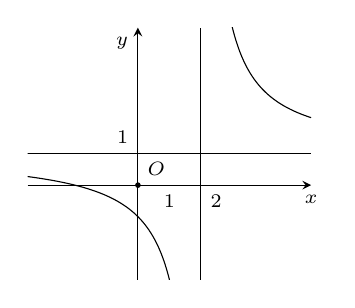
\begin{tikzpicture}[>=stealth,scale=0.4]
			\clip(-3.5,-3) rectangle (6,5);
			\draw[->,color=black] (-3.5,0.) -- (5.5,0.);
			\draw[->,color=black] (0.,-5) -- (0.,5);
			\draw (2,-5)--(2,5) (-5,1)--(5.5,1);
			\draw[smooth,samples=100,domain=-4.5:1.9] plot(\x,{(\x+2)/(\x-2)});
			\draw[smooth,samples=100,domain=2.1:5.5] plot(\x,{(\x+2)/(\x-2)});
			\draw (0,1) node[above left] {\scriptsize $1$};
			\draw (1,0) node[below] {\scriptsize $1$};
			\draw (2,0) node[below right] {\scriptsize $2$};
			\draw (5.5,0) node[below] {\scriptsize $x$};
			\draw (0,4.5) node[left] {\scriptsize $y$};
			\draw[fill=black] (0,0) circle (2pt) node[above right] {\scriptsize $O$};
	\end{tikzpicture}}
	\loigiai{
		Đồ thị của hàm số đã cho có đường tiệm cận đứng $x=-1$, tiệm cận ngang $y=1$ và đi qua các điểm $(0;-2),(2;0)$.}
\end{ex}
%%%==============EX_10============%%%
\begin{ex}%[2D1H5-7]
 Cho hàm số $g(x)$ liên tục trên $\mathbb{R}$ thỏa mãn $g'(0)=0$, $g''(x)<0$,  $\forall x \in (-1;2)$. Đồ thị của $g(x)$ là
	\choice
	{\True 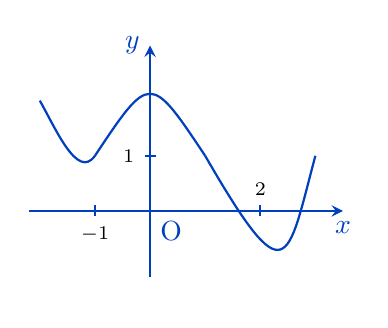
\begin{tikzpicture}[thick,blue!50!teal, scale=0.7]
			\draw[->,>=stealth] (-2.2,0)--(3.5,0) node[below]{$x$};
			\draw[->,>=stealth] (0,-1.2)--(0,3) node[left]{$y$};
			\draw (0,0) node[below right] {O};
			\draw (-1,0) --+(0,.1) 
			(-1,0)--+(0,-.1) node[below,black]{\scriptsize $-1$};
			\draw (2,0) --+(0,.1) node[above,black]{\scriptsize $2$} 
			(2,0)--+(0,-.1);
			\draw (0,1)--+(-.1,0) node[left,black]{\scriptsize $1$} 
			(0,1)--+(.1,0);
			% Vẽ đồ thị (tự chỉnh các tham số cho đến khi ưng ý)
			\draw (-2,2) to[out=-60,in=-125] (-1,1);
			\draw (-1,1) .. controls (0,2.5) .. (1,1);
			\draw (1,1) .. controls +(-60:3) and +(-105:2) .. (3,1);
	\end{tikzpicture}}
	{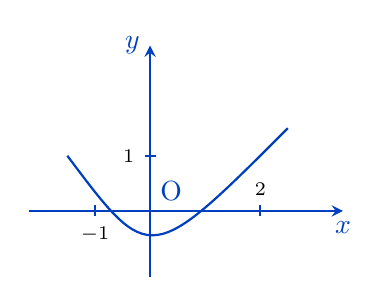
\begin{tikzpicture}[thick,blue!50!teal, scale=0.7]
			\draw[->,>=stealth] (-2.2,0)--(3.5,0) node[below]{$x$};
			\draw[->,>=stealth] (0,-1.2)--(0,3) node[left]{$y$};
			\draw (0,0) node[above right] {O};
			\draw (-1,0) --+(0,.1) 
			(-1,0)--+(0,-.1) node[below,black]{\scriptsize $-1$};
			\draw (2,0) --+(0,.1) node[above,black]{\scriptsize $2$} 
			(2,0)--+(0,-.1);
			\draw (0,1)--+(-.1,0) node[left,black]{\scriptsize $1$} 
			(0,1)--+(.1,0);
			% Vẽ đồ thị (tự chỉnh các tham số cho đến khi ưng ý)
			\draw (-1.5,1) .. controls (0,-1) .. (2.5,1.5);
	\end{tikzpicture}}
	{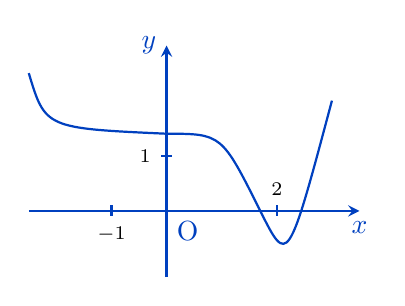
\begin{tikzpicture}[thick,blue!50!teal, scale=0.7]
			\draw[->,>=stealth] (-2.5,0)--(3.5,0) node[below]{$x$};
			\draw[->,>=stealth] (0,-1.2)--(0,3) node[left]{$y$};
			\draw (0,0) node[below right] {O};
			\draw (-1,0) --+(0,.1) 
			(-1,0)--+(0,-.1) node[below,black]{\scriptsize $-1$};
			\draw (2,0) --+(0,.1) node[above,black]{\scriptsize $2$} 
			(2,0)--+(0,-.1);
			\draw (0,1)--+(-.1,0) node[left,black]{\scriptsize $1$} 
			(0,1)--+(.1,0);
			% Vẽ đồ thị (tự chỉnh các tham số cho đến khi ưng ý)
			\draw (-2.5,2.5) .. controls (-2.2,1.5) .. (0,1.4);
			\draw (0,1.4) .. controls (1,1.4) .. (1.7,0);
			\draw (1.7,0) .. controls (2.2,-1) .. (3,2);
	\end{tikzpicture}}
	{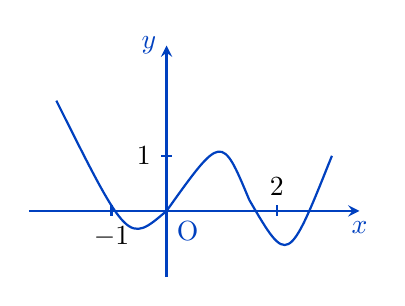
\begin{tikzpicture}[thick, blue!50!teal, scale=0.7]
			\draw[->,>=stealth] (-2.5,0)--(3.5,0) node[below]{$x$};
			\draw[->,>=stealth] (0,-1.2)--(0,3) node[left]{$y$};
			\draw (0,0) node[below right] {O};
			\draw (-1,0) --+(0,.1) 
			(-1,0)--+(0,-.1) node[below,black]{ $-1$};
			\draw (2,0) --+(0,.1) node[above,black]{ $2$} 
			(2,0)--+(0,-.1);
			\draw (0,1)--+(-.1,0) node[left,black]{ $1$} 
			(0,1)--+(.1,0);
			% Vẽ đồ thị (tự chỉnh các tham số cho đến khi ưng ý)
			\draw (-2,2) .. controls (-0.7,-0.6) .. (0,0);
			\draw (0,0) .. controls (1,1.4) .. (1.5,0.2);
			\draw (1.5,0.2) .. controls (2.2,-1) .. (3,1);
	\end{tikzpicture}}
	\loigiai{
		\immini{ Từ giả thiết $g'(0)=0$, $g''(x)<0$, $\forall x \in (-1;2)$  nên hàm số $g(x)$ đạt cực đại tại điểm $x=0$, do đó trong $4$ đồ thị đã cho, đồ thị có dạng như hình bên là đồ thị của hàm số $g(x)$.}
		{\hspace{2cm}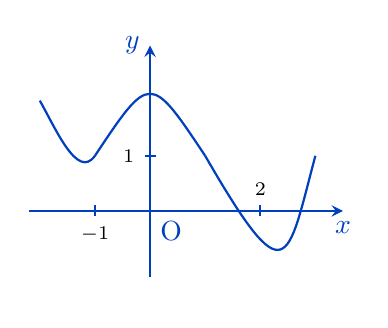
\begin{tikzpicture}[thick,blue!50!teal, scale=0.7]
				\draw[->,>=stealth] (-2.2,0)--(3.5,0) node[below]{$x$};
				\draw[->,>=stealth] (0,-1.2)--(0,3) node[left]{$y$};
				\draw (0,0) node[below right] {O};
				\draw (-1,0) --+(0,.1) 
				(-1,0)--+(0,-.1) node[below,black]{\scriptsize $-1$};
				\draw (2,0) --+(0,.1) node[above,black]{\scriptsize $2$} 
				(2,0)--+(0,-.1);
				\draw (0,1)--+(-.1,0) node[left,black]{\scriptsize $1$} 
				(0,1)--+(.1,0);
				% Vẽ đồ thị (tự chỉnh các tham số cho đến khi ưng ý)
				\draw (-2,2) to[out=-60,in=-125] (-1,1);
				\draw (-1,1) .. controls (0,2.5) .. (1,1);
				\draw (1,1) .. controls +(-60:3) and +(-105:2) .. (3,1);
		\end{tikzpicture}}
	}
\end{ex}
\Closesolutionfile{ans}
\indapan{6}{ans/ans-2-B4}

\cauds
\Opensolutionfile{ans}[ans/ans-2-B4-DS]
\begin{ex}%[ĐCHT-Toán12-GDPT2018, Lê Văn Hiếu]%[2D1B5-1]
	\immini{
		Hình vẽ sau là đồ thị của hàm số $y=\dfrac{ax+b}{cx+d}$. Xét tính đúng sai của các mệnh đề sau.
		\choiceTF
		{\True $ad>0$}
		{\True $bd<0$}
		{$ab>0$}
		{$ad-bc<0$}
	}{
		\begin{tikzpicture}[>=stealth',scale=0.5]
			\def\xmin{-5.5} \def\xmax{4}
			\def\ymin{-2.5} \def\ymax{6.5}
			\draw[domain=-5.5:4] plot(\x,{2});
			\draw[domain=-2.5:6.5,variable=\t] plot({-1},{(\t)});
			\draw[domain=-5.5:-1.67] plot(\x,{(2*(\x)-1)/((\x)+1)});
			\draw[domain=-0.33:4] plot(\x,{(2*(\x)-1)/((\x)+1)});
			\begin{scriptsize}
				\draw[->](\xmin,0)--(\xmax,0); \draw(\xmax-0.1,0) node[below]{$x$};
				\draw[->](0,\ymin)--(0,\ymax); \draw(0,\ymax-0.2) node[right]{$y$};
				\draw node [above left]{$O$};
			\end{scriptsize}
		\end{tikzpicture}
	}
	\loigiai{
		Dựa vào đồ thị hàm số ta thấy
		\begin{itemchoice}
			\itemch Đúng. Đồ thị hàm số có tiệm cận ngang $y=\dfrac{a}{c}>0$ và tiệm cận đứng $x=-\dfrac{d}{c}<0.$ Ta có $\heva{& \dfrac{a}{c}>0\\&\dfrac{d}{c}>0}\Rightarrow\dfrac{ad}{c^2}>0\Rightarrow ad>0$.
			\itemch Đúng. Đồ thị hàm số cắt trục $Oy$ tại điểm có tung độ nhỏ hơn $0\Rightarrow\dfrac{b}{d}<0\Rightarrow bd<0.$
			\itemch Sai. Từ $ad>0$ và $bd<0$ suy ra $adbd<0\Rightarrow ab<0$.
			\itemch Sai. Hàm số đã cho là hàm đồng biến trên mỗi khoảng xác định nên
						$$y'=\dfrac{ad-bc}{(cx+d)^2}>0\Rightarrow ad-bc>0.$$
		\end{itemchoice}
	}
\end{ex}
\begin{ex}%[ĐCHT-Toán12-GDPT2018, Lê Văn Hiếu]%[2D1B5-1]
	\immini{
		Cho hàm số $y=\dfrac{(a-1)x+b}{(c-1)x+d}$, $d<0$ có đồ thị như hình vẽ. Xét tính đúng sai của các khẳng định dưới đây.
		\choiceTF
		{$a>1, b>0, c<1$}
		{$a>1, b<0, c>1$}
		{$a<1, b>0, c<1$}
		{\True $a>1, b>0, c>1$}
	}{
		\begin{tikzpicture}[scale=1, font=\footnotesize, line join=round, line cap=round,>=stealth]
			\def\a{1} \def\b{1} \def\c{2} \def\d{-1} % Hệ số
			\def\xmin{-2} \def\xmax{3}
			\def\ymin{-2} \def\ymax{3}
			\draw[->] (\xmin,0)--(\xmax,0) node [below]{$x$};
			\draw[->] (0,\ymin)--(0,\ymax) node [left]{$y$};
			\node at (0,0) [above left]{$O$};
			\clip (\xmin+0.1,\ymin+0.1) rectangle (\xmax-0.1,\ymax-0.1);
			\draw[smooth,samples=300,domain=\xmin:(-\d/\c-0.1)] plot(\x,{(\a*(\x)+\b)/(\c*(\x)+\d)});
			\draw[smooth,samples=300,domain=(-\d/\c+0.1:\xmax)] plot(\x,{(\a*(\x)+\b)/(\c*(\x)+\d)});
			\draw[dashed] (-\d/\c,\ymin)--(-\d/\c,\ymax);
			\draw[dashed] (\xmin,\a/\c)--(\xmax,\a/\c);
		\end{tikzpicture}
	}
	\loigiai{
		Theo bài ra, đường tiệm cận đứng của đồ thị hàm số là $x=-\dfrac{d}{c-1}$.\\
		Đường tiệm cận ngang của đồ thị hàm số là $y=\dfrac{a-1}{c-1}$.\\
		Nhìn đồ thị ta thấy: $x=-\dfrac{d}{c-1}>0$ mà $d<0\Rightarrow c-1>0\Rightarrow c>1$.\\
		$y=\dfrac{a-1}{c-1}>0\Rightarrow a-1>0\Rightarrow a>1$.\\
		Đồ thị cắt trục tung tại điểm có tung độ bằng $\dfrac{b}{d}<0\Rightarrow b>0$.
		\begin{itemchoice}
			\itemch Sai
			\itemch Sai
			\itemch Sai
			\itemch Đúng
		\end{itemchoice}
	}
\end{ex}

\begin{ex}%[ĐCHT-Toán12-GDPT2018, Lê Văn Hiếu]%[2D1B5-1]
	\immini{
		Cho hàm số $y=ax^3+bx^2+cx+d$ có đồ thị như hình bên. Xét tính đúng sai của các mệnh đề sau.
		\choiceTF
		{\True $ad>0$}
		{\True $bc>0$}
		{$ad<0$}
		{$abc<0$}
	}{
		\begin{tikzpicture}[scale=1, font=\footnotesize, line join=round, line cap=round,>=stealth]
			\def\a{0.5}  % Hệ số co dãn
			\def\xmin{-1.3} \def\xmax{4}
			\def\ymin{-2.5} \def\ymax{2} 
			\draw[->] (\xmin,0)--(\xmax,0) node [below]{$x$};
			\draw[->] (0,\ymin)--(0,\ymax) node [left]{$y$};
			\node at (0,0) [below left]{$O$};
			\clip (\xmin+0.1,\ymin+0.1) rectangle (\xmax-0.1,\ymax-0.1);
			\draw[smooth,samples=300] plot(\x,{\a*((\x+0.8)*(\x-0.6)*(\x-3))});
		\end{tikzpicture}
	}
	\loigiai{
		\begin{itemchoice}
			\itemch Đúng. Từ dáng điệu của đồ thị ta có
			\begin{itemize}
				\item $\lim\limits_{x\to+\infty} y=+\infty;\lim\limits_{x\to-\infty} y=-\infty\Rightarrow a>0$.
				\item  Đồ thị hàm số cắt trục tung tại một điểm có tung độ dương nên $d>0$.
			\end{itemize}
			Suy ra $ad>0$.
			\itemch Đúng. Ta có $y'=3ax^2+2bx+c$.\\
			Mặt khác dựa vào đồ thị ta thấy phương trình $y'=0$ có hai nghiệm trái dấu và tổng hai nghiệm này luôn dương nên $\heva{&ac<0\\&-\dfrac{2b}{3a}>0}\Rightarrow ac\cdot\left(-\dfrac{2b}{3a}\right)<0$ hay $bc>0$.
			\itemch Sai. $ad>0$ (đã chỉ ra).
			\itemch Sai. Từ lập luận trên ta có $a>0$, $b<0$ và $c<0$ nên $abc>0$.
		\end{itemchoice}
	}
\end{ex}
\begin{ex}%[ĐCHT-Toán12-GDPT2018, Lê Văn Hiếu]%[2D1B5-1]
	\immini{
		Cho hàm số $y=\dfrac{ax^2+bx+c}{mx+n}$ có đồ thị như hình vẽ bên. Xét tính đúng sai của các khẳng định sau.
		\choiceTF
		{\True Hàm số có $2$ cực trị}
		{$x_\text{CĐ}=-2$}
		{$\dfrac{n}{m}=-1$}
		{\True Đồ thị hàm số có tâm đối xứng là $I(-1,2)$}
	}{\begin{tikzpicture}[line cap=butt,line join=miter,>=stealth,scale=0.5,font=\tiny]
			\tikzset{declare function={xmin=-6.2;xmax=4.8;ymin=-4.6;ymax=7.8;},
				smooth,samples=450}
			\draw[->] (xmin,0)--(xmax,0) node[shift={(0:7pt)}]{$ x $};
			\draw[->] (0,ymin)--(0,ymax) node[shift={(90:7pt)}]{$ y $};
			\fill (0,0) node[shift={(140:5pt)}]{$O$};
			\clip (xmin,ymin-.7) rectangle (xmax,ymax);
			\foreach\i in {-2,2}{\draw(\i,1.5pt)--(\i,-1.5pt)node[below]{$\i$};}
			\foreach\j in {-2,2,4}{\draw(-1.5pt,\j)--(1.5pt,\j) node[right]{$\j$};}
			\def\f(#1){(-(#1)^2)/((#1)+1)} % Hàm số
			\def\q(#1){(-(#1)+1)} % Tiệm cận xiên
			\def\a{0}
			\def\b{-2}
			\pgfmathsetmacro\fa{\f(\a)}
			\pgfmathsetmacro\fb{\f(\b)}
			\draw[samples=250] plot[domain=-7.4:-1.1] (\x,{\f(\x)});
			\draw[samples=250] plot[domain=-0.9:15] (\x,{\f(\x)});
			\draw[] plot [domain=-7.4:7] (\x,{\q(\x)}) ;
			\draw[] (-1,ymin)--(-1,ymax) node[sloped,pos=0.9,below] {$x=-1$};
			\foreach\x/\y in {\a/\fa,\b/\fb}{
				\draw[dashed] (\x,0)|-(0,\y);}
			\foreach\x/\y in {\a/\fa,\b/\fb}{\fill[white,draw=black] (\x,\y) circle (1pt);}
		%	\fill[white,draw=black] (-1,2) circle (1pt) node[text=black,shift={(14pt,5pt)}] {$I $};
		%	\node at (-1,-5) [right,fill=white,font=\footnotesize]{\it Hình LT $5$};
	\end{tikzpicture}}
	\loigiai{
		\begin{itemchoice}
			\itemch Đúng. Dựa vào đồ thị hàm số có hai điểm cực trị.
			\itemch Sai. Vì $x_\text{CĐ}=0$.
			\itemch Sai. Tiệm cận đứng của đồ thị là $x=-\dfrac{n}{m}=-1\Rightarrow \dfrac nm=1$.
			\itemch Đúng. Đồ thị hàm số có tâm đối xứng là $I(-1,2)$.
		\end{itemchoice}
	}
\end{ex}
%%%TLN
\Closesolutionfile{ans}
\indapan{3}{ans/ans-2-B4-DS}

\Opensolutionfile{ans}[ans/ans-2-B4-KQ]
\caukq
\begin{ex}%[ĐCHT-Toán12-GDPT2018, Lê Văn Hiếu]%[2D1B5-1]
	\immini{
		Hình bên là đồ thị của hàm số $y=\dfrac{ax+b}{x+c}$ (với $a,b,c\in\mathbb{R}$). Khi đó $ab-c$ bằng bao nhiêu?
	}{
		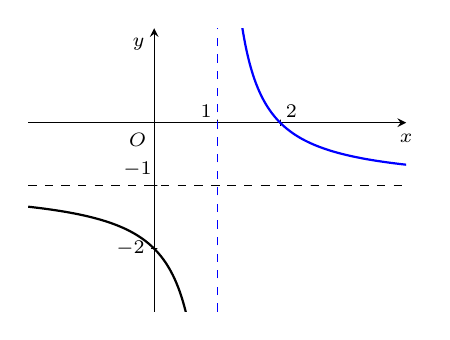
\begin{tikzpicture}[>=stealth, scale=.8]
			\def\xmin{-2}\def\xmax{4}\def\ymin{-3}\def\ymax{1.5}
			\draw[->](\xmin,0)--(\xmax,0)node [shift={(-90:.2)},scale=1]{\scriptsize $x$};
			\draw[->](0,\ymin)--(0,\ymax)node [below left] {\scriptsize $y$};
			\clip(\xmin,\ymin) rectangle (\xmax,\ymax);
			\foreach \p/\g in {1/135,2/45}\draw(\p,0)node[shift={(\g:.2)},scale=1]{\scriptsize $\p$}--+(0,.05)--+(0,-.05);
			\foreach \p/\g in {-2/180,-1/135}\draw(0,\p)node[shift={(\g:.3)},scale=1]{\scriptsize $\p$}--+(.05,0)--+(-.05,0);
			\foreach \p/\g in {0/-135}\draw(0,\p)node[shift={(\g:.3)},scale=1]{\scriptsize $O$};
			\draw[thick,smooth,samples=100] plot[domain=\xmin:0.99](\x,{(-\x+2)/(\x-1)})node[left]{\scriptsize };
			\draw[thick,blue,smooth,samples=100] plot[domain=1.01:\xmax](\x,{(-\x+2)/(\x-1)})node[left]{\scriptsize };
			\draw[dashed,smooth,samples=100] plot[domain=\xmin:\xmax](\x,{-1})node[left]{\scriptsize };
			\draw[dashed,blue,smooth,samples=100](1,\ymin)--(1,\ymax);
		\end{tikzpicture}
	}
	\loigiai{
		Đồ thị có tiệm cận đứng là $x=1$. Suy ra $-c=1 \Rightarrow c=-1$.\\
		Đồ thị có tiệm cận ngang $y=-1\Rightarrow a=-1$.\\
		Mặt khác, $y(0)=-2\Leftrightarrow \dfrac bc=-2\Rightarrow b=2$.\\
		Vậy, $ab-c=-2-(-1)=-1$.
		\shortans{$-1$}
	}
	
\end{ex}

\begin{ex}%[ĐCHT-Toán12-GDPT2018, Lê Văn Hiếu]%[2D1K5-1]
	\immini{
		Cho hàm số $y=f(x)=ax^3+bx^2+cx+d$ có đồ thị $(C)$ như hình vẽ. Khi đó $f(5)$ bằng
	}{
		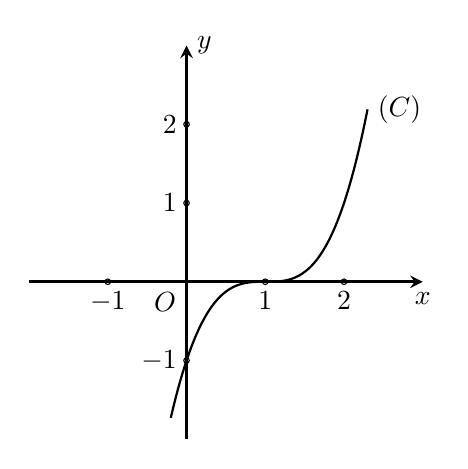
\begin{tikzpicture}[>=stealth]
			\draw[->,line width = 1pt] (-2,0)--(0,0) node[below left]{$O$}--(3,0) node[below]{$x$};
			\draw[->,line width = 1pt] (0,-2) --(0,3) node[right]{$y$};
			\foreach \x in {-1,1,2}{
				\draw (\x,0) node[below]{$\x$} circle (1pt);
				\draw (0,\x) node[left]{$\x$} circle (1pt);
			}
			\draw [black, thick, domain=-0.2:2.3, samples=100] %
			plot (\x, {(\x)^3-3*(\x)^2+3*(\x)-1}) node[right]{$(C)$};
		\end{tikzpicture}
	}
	\loigiai{
		Gọi hàm số bậc $3$ cần tìm có dạng là $y=ax^3+bx^2+cx+d \Rightarrow y' = 3ax^2+ 2bx + c$. Từ đồ thị ta có
		$$\heva{&d=-1\\&a+b+c+d=0\\&3a+2b+c=0\\&b^2-3ac=0}\Leftrightarrow\heva{&a=1\\&b=-3\\&c=3\\&d=-1}\Rightarrow y=x^3-3x^2+3x-1.$$
		Suy ra $f(5)=64$.
		\shortans{$64$}
	}
	
\end{ex}

\begin{ex}%[ĐCHT-Toán12-GDPT2018, Lê Văn Hiếu]%[2D1B5-1]
	\immini{
		Cho hàm số $ y=\dfrac{ax+2}{cx+d}$ có đồ thị như hình vẽ. Tích $acd$ bằng bao nhiêu?
	}{
		\begin{tikzpicture}[>=stealth,scale=.5]
			\def\xmin{-4}\def\xmax{10}\def\ymin{-3}\def\ymax{5}
			\draw[->](\xmin,0)--(\xmax,0)node [shift={(-90:.2)},scale=1]{\scriptsize $x$};
			\draw[->](0,\ymin)--(0,\ymax)node [below right] {\scriptsize $y$};
			\clip(\xmin,\ymin) rectangle (\xmax,\ymax);
			\foreach \p/\g/\a in {0/-45/O, 3/-45/3, -2/-90/-2}\draw(\p,0)node[shift={(\g:.2)},scale=1]{\scriptsize $\a$}--+(0,.05)--+(0,-.05);
			\foreach \p/\g in {-1/180,1/120}\draw(0,\p)node[shift={(\g:.3)},scale=1]{\scriptsize $\p$}--+(.05,0)--+(-.05,0);
			\draw[smooth,samples=100] plot[domain=\xmin:2.99](\x,{((\x)+2)/(\x-3)})node[left]{\scriptsize};
			\draw[smooth,samples=100] plot[domain=3.01:\xmax](\x,{((\x)+2)/(\x-3)})node[left]{\scriptsize};
			\draw(\xmin,1)--(\xmax,1)(3,\ymin)--(3,\ymax);
		\end{tikzpicture}
	}
	\loigiai{
		Nhìn vào đồ thị hàm số, ta thấy:
		\begin{itemize}
			\item Đồ thị hàm số cắt $Ox$ tại điểm có hoành độ bằng $-2$, nên $\dfrac{-2}{a}=-2$, do đó $ a=1$.
			\item Đồ thị hàm số có đường tiệm cận ngang là $ y=\dfrac{a}{c}=1$, mà $ a=1$, do đó $ c=1$.
			\item Đồ thị hàm số có đường tiệm cận đứng là $ x=-\dfrac{d}{c}=3$, mà $ c=1$, do đó $ d=-3$.
		\end{itemize}
		Vậy, $acd=1\cdot1\cdot(-3)=-3$.
		\shortans{$-3$}
	}
	
\end{ex}


\begin{ex}%[ĐCHT-Toán12-GDPT2018, Lê Văn Hiếu]%[2D1K5-1]
	\immini{
		Cho hàm số bậc ba $y=ax^3+bx^2+cx+d$ có đồ thị như hình vẽ. Tìm giá trị nhỏ nhất của biểu thức $P=a^2+c^2+b+1$. (Kết quả làm tròn đến hàng phần trăm).
	}{
		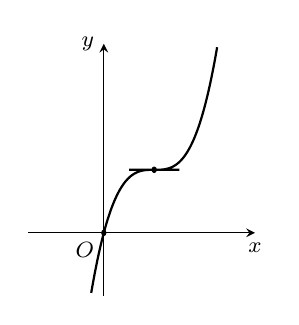
\begin{tikzpicture}[>=stealth,font=\footnotesize,xscale=.8,scale=.8]
			\draw[->] (-1.5,0)--(3,0)node[below]{$x$};
			\draw[->] (0,-1)--(0,3)node[left]{$y$};
			\draw[thick] plot[smooth,samples=100,domain=-.25:2.25] (\x,{(\x-1)^3+1}) (1-.5,1)--(1+.5,1);
			\fill (1,1)circle(1.5pt) (0,0)node[below left]{$O$}circle(1.5pt);
		\end{tikzpicture}
	}
	\loigiai{
		Ta có $y'=3ax^2+2bx+c$. Từ đồ thị suy ra $d=0$, $b^2-3ac=0\Rightarrow ac=\dfrac{b^2}{3}$.\\
		Do đó, $P\ge 2ac+b+1=\dfrac{2b^2}{3}+b+1=\dfrac{2}{3}\left(b+\dfrac{3}{4}\right)^2+\dfrac{5}{8}\ge \dfrac{5}{8}$.\\
		Vậy $\min P=\dfrac{5}{8}\approx 0{,}63$ tương ứng với $a=c=\dfrac{\sqrt{3}}{4},b=-\dfrac{3}{4}$.
		\shortans{$0{,}63$}
	}
	
\end{ex}

\begin{ex}%[ĐCHT-Toán12-GDPT2018, Lê Văn Hiếu]%[2D1K5-1]
	\immini{
		Cho hàm số bậc ba $f(x)=x^3+bx^2+cx+d$. Biết đồ thị của hàm số $y=f'(x)$ như hình vẽ. Giá trị của $\dfrac{c}{b}$ là (làm tròn đến hàng phần chục)
	}{
		\begin{tikzpicture}[scale=1,>=stealth, font=\footnotesize, line join=round, line cap=round]
			\def\a{1} \def\b{-2} \def\c{0.75} % Hệ số
			\def\xmin{-1} \def\xmax{2.5}
			\def\ymin{-1} \def\ymax{2}
			\draw[->] (\xmin,0)--(\xmax,0) node [below]{$x$};
			\draw[->] (0,\ymin)--(0,\ymax) node [left]{$y$};
			\node at (0,0) [below left]{$O$};
			\fill [black] (1,0) node[above]{$1$} circle (1.2pt);
			\fill [black] (0.5,0) node[below]{$\dfrac{1}{2}$} circle (1.2pt);
			\fill [black] (1.5,0) node[below]{$\dfrac{3}{2}$} circle (1.2pt);
			\clip (\xmin+0.1,\ymin+0.1) rectangle (\xmax-0.5,\ymax-0.1);
			\draw[smooth,samples=300] plot(\x,{\a*(\x)^2+\b*(\x)+\c});
		\end{tikzpicture}
	}
	\loigiai{
		Tập xác định $\mathscr{D}=\mathbb{R}$.\\
		Đạo hàm cấp $1$ của $f(x)$ là $f'(x)=3ax^2+2bx+c$.\\
		Dựa vào đồ thị của hàm số $f'(x)$ ta có bảng biến thiên của hàm số $f(x)$ như sau:
		\begin{center}
			
\begin{tikzpicture}
				\tkzTabInit[espcl=2.5,lgt=1.5,nocadre=false]
				{$x$/1,$f'(x)$/0.7,$f(x)$/2.1}
				{$-\infty$,$\dfrac{1}{2}$,$\dfrac{3}{2}$,$+\infty$}
				\tkzTabLine{,+,0,-,0,+,}
				\tkzTabVar{-/$-\infty$,+/$f\left(\tfrac{1}{2} \right) $,-/$f\left(\tfrac{3}{2} \right)$,+/$+\infty$}
			\end{tikzpicture}
		\end{center}
		Ta có $f'\left(\dfrac{1}{2}\right)=\dfrac{3a}{4}+b+c$ và $f'\left(\dfrac{3}{2}\right)=\dfrac{27a}{4}+3b+c$.\\
		Dựa vào bảng biến thiên ta có 
		$$\heva{&3a+4b+4c=0\\&27a+12b+4c=0} \Leftrightarrow \heva{&27a+36b+36c=0\\&27a+12b+4c=0}
		\Rightarrow 24b+32c=0 \Rightarrow \dfrac{c}{b}=-\dfrac{3}{4}.$$\\
		Vậy $\dfrac{c}{b}=-\dfrac{3}{4}\approx-0{,}8$.
		\shortans{$-0{,}8$}
	}
	
\end{ex}
\begin{ex}
	Cho đồ thị hàm số $y=5x-1+\dfrac{8}{x-1}$ có tâm đối xứng $I(a;b)$. Giá trị của biểu thức $C=a+3b$.
	\loigiai{
		Hàm số đã cho có tiệm cận đứng là $x=1$ và tiệm cận xiên $y=5x-1$ nên tâm đối xứng của đồ thị là $I(1;4)$. Vậy $C=13$.
		\shortans{$13$}
	}
	\end{ex}
\Closesolutionfile{ans}
\indapan{6}{ans/ans-2-B4-KQ}